\chapter{Verification and Results}
\label{chap:results}
The previous chapters described how the LLVM-based $\rho$-VEX compiler has been implemented. In this chapter we are going to verify the correct operation of the compiler and we are going to measure the performance of the binaries that are generated with the LLVM-based compiler. 

\section{Verification}
Unit testing has been used to verify the correct operation of the LLVM compiler. The tests have been performed using the XSTsim simulator. XSTsim can only print pipeline and register information to the terminal. It is not possible to parse strings or information from the program that is executing back to the user. To check if tests are executed correctly we check the return statement after execution of a benchmark. The value in the return register indicates wheter the test executed correclty or where at which point the test failed.

\begin{itemize}
	\item \textbf{arit.c:} Integer arithmetic tests for \texttt{char}, \texttt{short}, \texttt{int} and \texttt{long long}.
	\item \textbf{if.c:} Integer and boolean comparison operators.
	\item \textbf{float.c:} Testing of floating point library.
	\item \textbf{func.c:} Tests involving pointers and structures.
	\item \textbf{global.c:}  Tests involving global integers, arrays and structures.
	\item \textbf{call.c:} Function calls.
	\item \textbf{func\_pointer.c:} Function calls using function pointers.
	\item \textbf{loop.c:} Basic while loops.
	\item \textbf{misc.c:} Others tests.
\end{itemize}

During preliminary testing of the benchmark additional errors have been found. The verification tests have been updated to catch these errors. Unfortunately some benchmarking errors are not possible to define as a unit test. Some errors, such as scheduling and register allocation errors, only occur in complex programs. Translating these errors to simple unit tests is not possible because they depend on the higher-level structure of the program.

\section{Benchmark results}
The powerstone benchmark \cite{Jeff-Scott:1998fj} has been used to evaluate the performance of the LLVM-based compiler. The benchmarks consist of a number of programs that test certain functionality. In addition to performance evaluation the benchmarks are also useful to check the executable correctness of the generated binaries.

Benchmarking can be performed using the architecture simulator XSTsim and using the hardware simulator. We have chosen to use the Modelsim hardware simulator because a complete logical simulation of the processor is used for evaluation. Modelsim builds a simulation environment using the $\rho$-VEX VHDL files. A testbench is used to generate test signals. For this simulation the testbench is used to load the instruction and data memory of the $\rho$-VEX processor and to generate correct clock and enable signals to start execution. In Figure \ref{fig:rvex_tb} the testbench process is displayed.

\begin{figure}[ht]
\centering
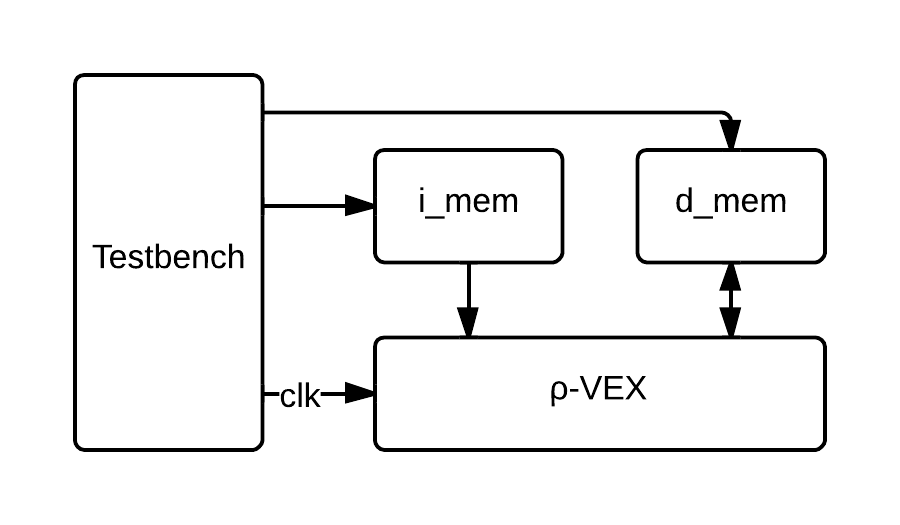
\includegraphics[width=0.8\textwidth]{5_results/img/testbench.png}
\caption{$\rho$-VEX testbench}
\label{fig:rvex_tb}
\end{figure}

Modelsim wave viewer can be used to monitor execution of the processor. The wave viewer has been used to check the contents of the registers and to monitor the instruction pipeline when necessary.

The architectural simulator has not been used because it only operates on a description of the $\rho$-VEX processor. Bugs that are present in the architectural simulator are not necessarily present in the actual processor. By using the Modelsim simulator we can be sure to a reasonable extent that binaries that execute in Modelsim will also execute on actual hardware. 

The following benchmarks have been used for evaluation:

\begin{itemize}
	\item \textbf{adpcm:} codec for voice compression.
	\item \textbf{bcnt:} Bitwise shift and operations on 1K array.
	\item \textbf{blit:} Graphics application
	\item \textbf{compress:} UNIX compression utility
	\item \textbf{crc:} Cyclic redundancy check.
	\item \textbf{engine:} Engine control application
	\item \textbf{g3fax:} Group 3 fax decode.
	\item \textbf{matrix:} Matrix multiplication.
	\item \textbf{pocsag:} Communication protocol for paging applications.
	\item \textbf{ucbqsort:} Quicksort algorithm.
\end{itemize}

Unfortunately not all benchmarks execute correctly. Currently all benchmarks work on the XSTsim simulator but some benchmarks do not work correctly using the Modelsim simulator. This indicates possible bugs in the LLVM-based compiler that are probably related to scheduling errors. XSTsim has proven to be less strict when executing instructions with different latencies. Problems have been found with the following benchmarks:

\begin{itemize}
	\item \textbf{fir:} Unclear how program operates. Omitted because benchmark was also unable to compile on X86 based systems.
	\item \textbf{jpeg:} Output not correct. Output is very close to expected value so this probably indicates a minor error in the compiler.
	\item \textbf{qurt:} Infinite loop.
	\item \textbf{des:} No check on output so impossible to determine if execution was correct.
	\item \textbf{v42:} Output not correct.
\end{itemize}

\subsection{General performance}
General performance of all the compilers that target the $\rho$-VEX processor are shown in Tables \ref{tbl:LLVM_perf}, \ref{tbl:HP_perf} and \ref{tbl:GCC_perf}. As expected the HP-based compiler performs excellent but unfortunately is not able to produces correct executables for higher issue widths. The GCC compiler has only been implemented for a 4 issue width $\rho$-VEX processor.

The absolute performance of the compilers is displayed in Figure \ref{fig:abs_perf}. As expected the HP-based compiler generates the best performing binaries. The LLVM-based compiler offers some speed improvements over the GGC-based compiler for most benchmarks. 

The HP-based compiler generates excellent performing binaries because it has a superiour scheduling techniques for finding and extracting ILP in source code. The HP-based compiler uses a trace based scheduling technique which enables better ILP extraction. In addition to this the HP-based compiler also seems to do more optimization. Even when compiling with \texttt{-O0} the compiler already performs certain optimizations that are not available for LLVM-based compiler. For example, compare the output for the following simple C program:

\begin{lstlisting}[language=c]
int main() {
	int a = 3, b = 2, c;

	c = a + b;

	return c;
}
	
\end{lstlisting}

Listing \ref{lst:hp_ex} displays the output of the HP-based compiler and Listing \ref{lst:llvm_ex} shows the output of the LLVM-based compiler. The output shows immediatly that the HP-based compiler has eliminated the add operation and has copied the final value of the operation straight to the return register. The LLVM compiler is only able to perform these kind of operations at higher optimization levels.

\begin{lstlisting}[language=rvex,label=lst:hp_ex, caption={HP compiler output}]

	add $r0.3   = $r0.0, 5  	## Move to return register
;;
	return
;;
\end{lstlisting}

\begin{lstlisting}[language=rvex,label=lst:llvm_ex, caption={LLVM compiler output}]

	add $r0.2 	= $r0.0, 2
	add $r0.3 	= $r0.0, 3	
;;
	add $r0.3   = $r0.2, $r0.3  ## Move to return register
;;
	return
;;
\end{lstlisting}

Close inspection of the absolute performance reveals some interesting facts related to the issue width of the processor. Increasing the issue width from 2 issue to 4 issue leads to a significant increase in performance. Further increasing the issue width to 8 issue machine does not lead to an increase in performance. This is shown in Figure \ref{fig:rel_issue}. For some benchmarks such as \texttt{bcnt} the LLVM-based compiler is able to find extra parallelism but for most benchmarks the performance increase is non-existent.

Manual inspection of the assembly files that are generated shows that both compilers are able to generate instruction packets that use a higher number of functional units. These large instruction packets do not lead to an increase in performance because they are not contained inside loop structures. The amount of times large instruction packets are executed is limited. 


\begin{figure}[ht]
\centering
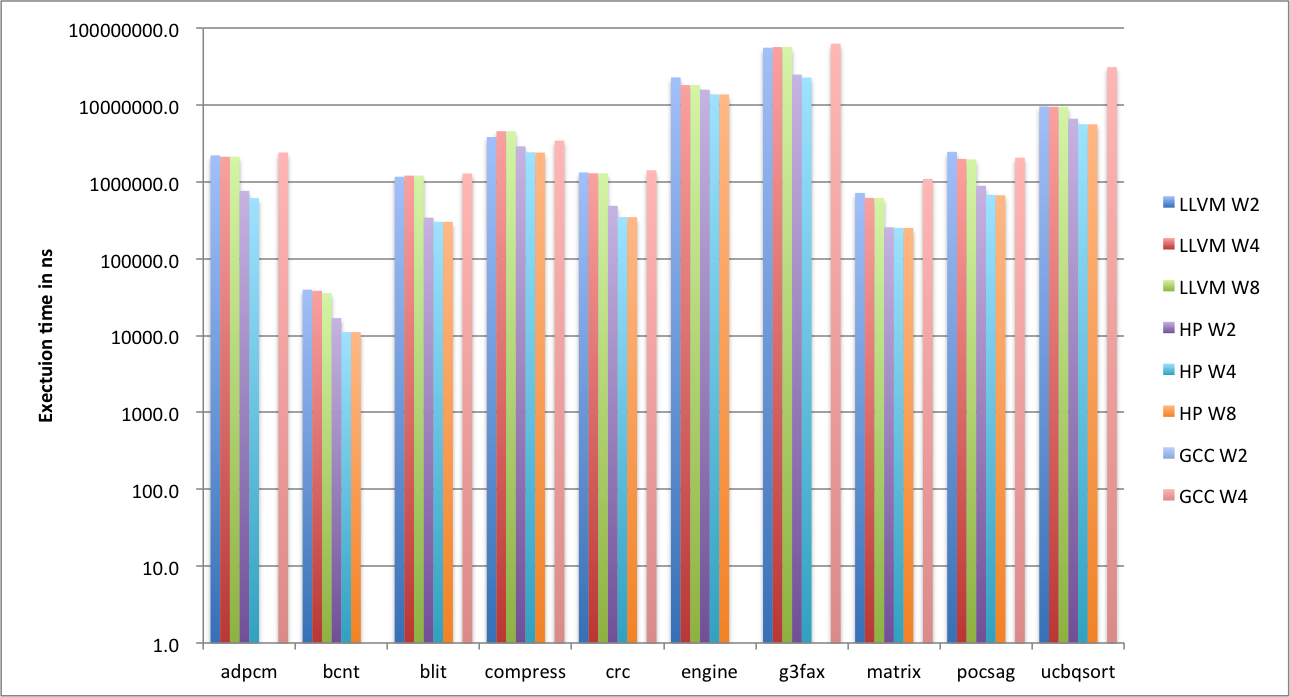
\includegraphics[width=0.8\textwidth]{5_results/img/abs_perf.png}
\caption{Absolute performance}
\label{fig:abs_perf}
\end{figure}

\begin{figure}[ht]
\centering
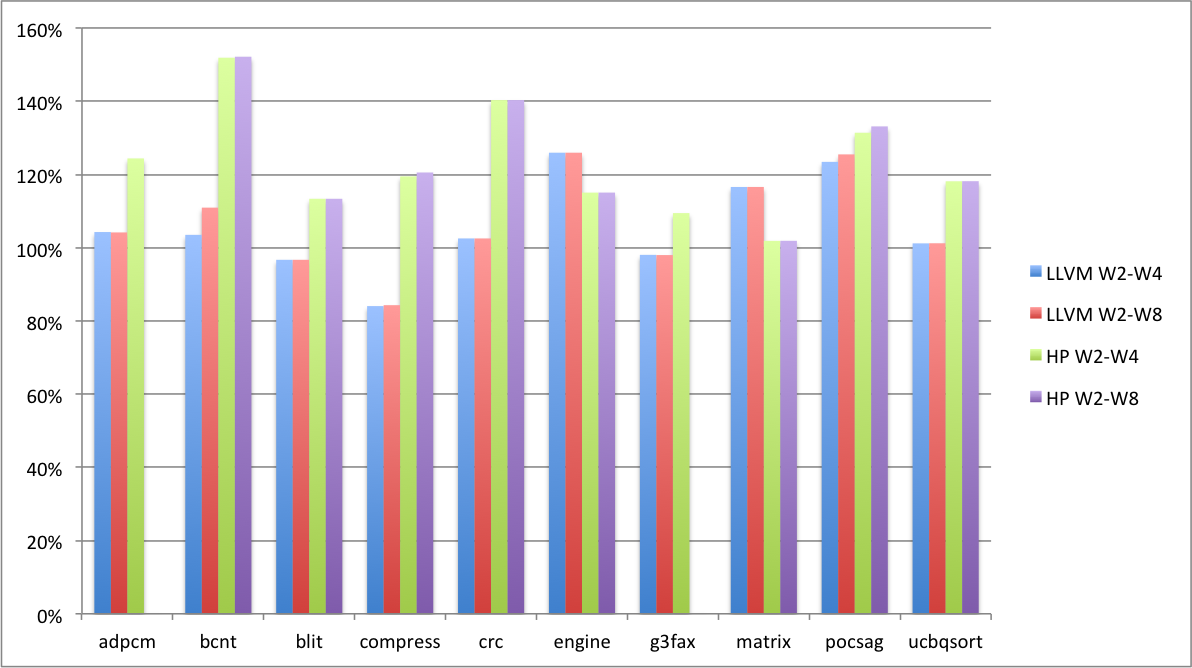
\includegraphics[width=0.8\textwidth]{5_results/img/rel_issue.png}
\caption{Relative performance for increasing issue width}
\label{fig:rel_issue}
\end{figure}

Figure \ref{fig:rel_HP} shows the relative performance of LLVM-based binaries compared to HP-based binaries. Higher then 100\% indicates LLVM-based binaries performing better then HP-based binaries. As expected HP-based binaries perform better then LLVM-based binaries. Inspection of the generated assembly files indicate that the HP-based compiler is able to fill significantly more functional units then the LLVM-based compiler. Further the LLVM-based compiler is overly aggressive in inserting nop instructions to reduce structural and data hazards.


\begin{figure}[ht]
\centering
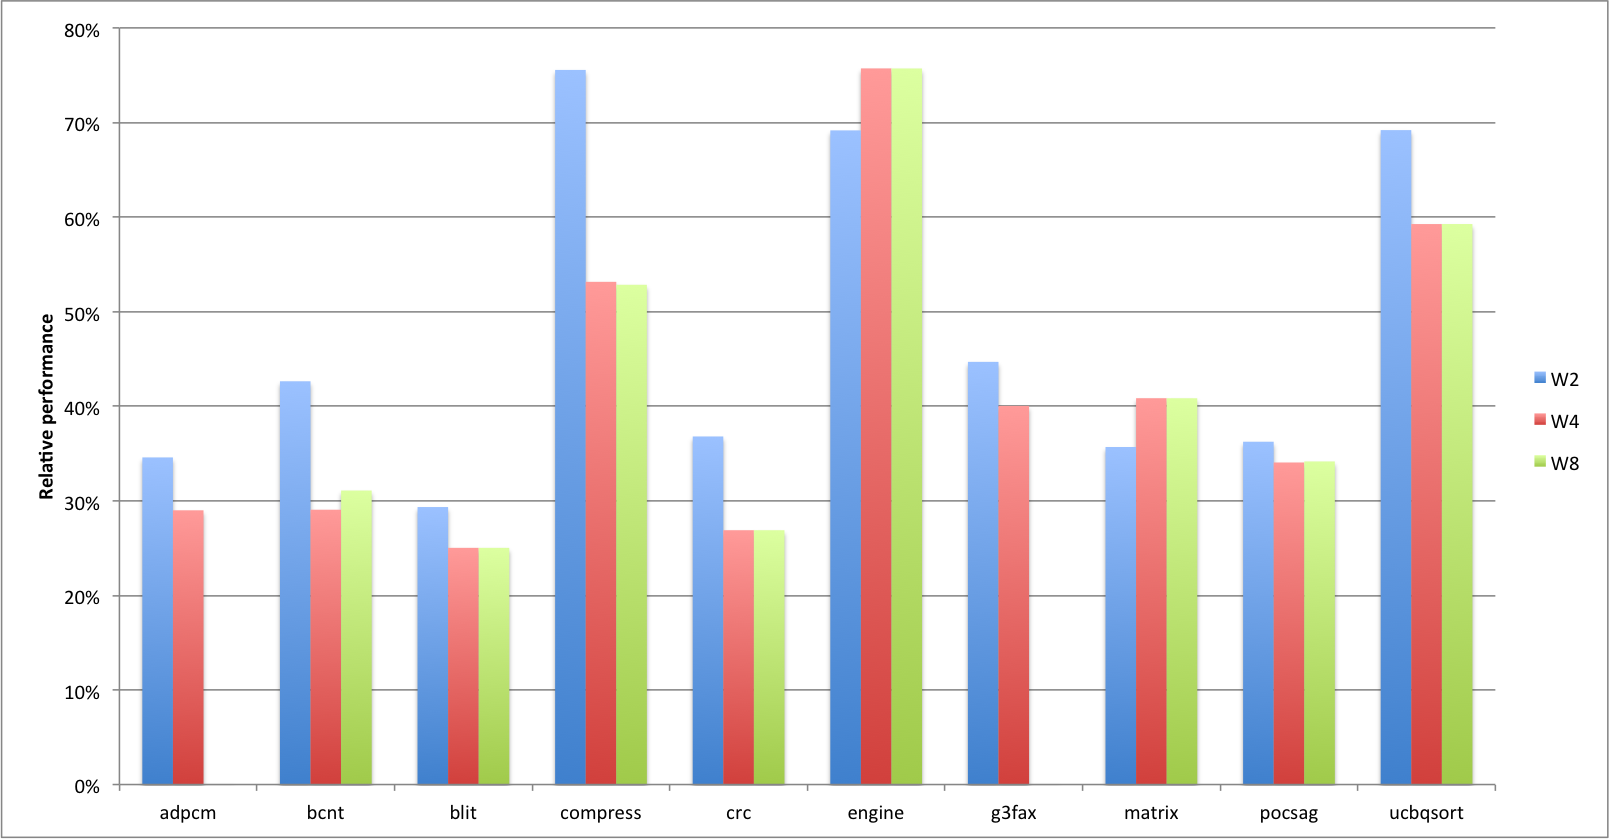
\includegraphics[width=0.8\textwidth]{5_results/img/rel_HP.png}
\caption{HP-LLVM relative performance}
\label{fig:rel_HP}
\end{figure}

Figure \ref{fig:rel_GCC} shows the relative performance of LLVM-based binaries compared to GCC-based binaries. Performance of the LLVM-based compiler shows mixed results. Some benchmarks perform significantly better such as \texttt{matrix} and \texttt{ucbqsort} but both compress and pocsag perform worse. Manual inspection of these benchmark do not show a big reason for decreased performance except for the overly aggressive \texttt{nop} insertion of the LLVM machine scheduler.

\begin{figure}[ht]
\centering
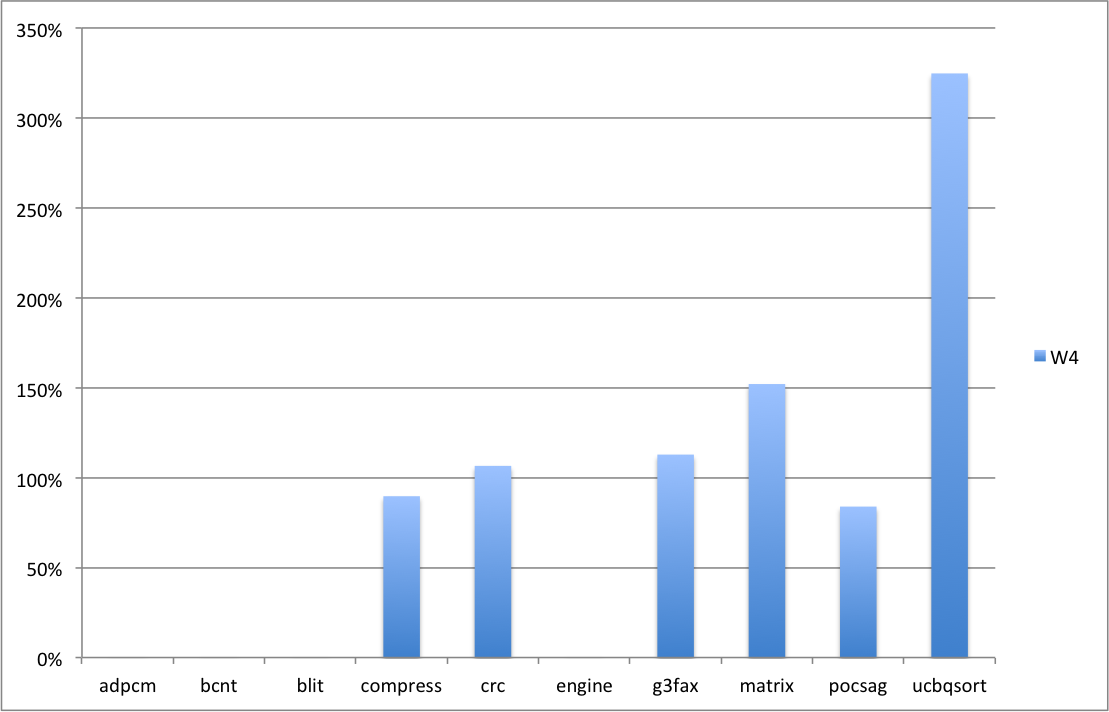
\includegraphics[width=0.8\textwidth]{5_results/img/rel_GCC.png}
\caption{GCC-LLVM relative performance}
\label{fig:rel_GCC}
\end{figure}


\begin{table}
  \centering
    \begin{tabular}{|l|r|r|r|}
    \hline
    \textbf{Benchmark} & \multicolumn{1}{|r|}{\textbf{W2}} & \multicolumn{1}{|r|}{\textbf{W4}}  & \multicolumn{1}{|r|}{\textbf{W8}} \\ \hline
	\texttt{adpcm} 		&  2.206.300	&  2.115.820 	&  2.118.040 	\\ \hline
	\texttt{bcnt} 		&  39.540		&  38.200 		&  35.640 		\\ \hline
	\texttt{blit} 		&  1.164.280	&  1.204.140 	&  1.204.120 	\\ \hline
	\texttt{compress} 	&  3.828.700	&  4.555.420 	&  4.541.900 	\\ \hline
	\texttt{crc} 		&  1.323.160	&  1.290.540 	&  1.290.560 	\\ \hline
	\texttt{engine} 	&  22.820.980	&  18.119.680 	&  18.119.680 	\\ \hline
	\texttt{g3fax} 		&  55.537.540	&  56.645.740 	&  56.680.260 	\\ \hline
	\texttt{matrix} 	&  717.100		&  615.060 		&  615.040 		\\ \hline
	\texttt{pocsag} 	&  2.453.040	&  1.987.140 	&  1.954.860 	\\ \hline
	\texttt{ucbqsort} 	&  9.568.680	&  9.457.160 	&  9.454.600 	\\ \hline
    \end{tabular}
  \caption{LLVM-based compiler performance in ns}
  \label{tbl:LLVM_perf}
\end{table}

\begin{table}
  \centering
    \begin{tabular}{|l|r|r|r|l|}
    \hline
    \textbf{Benchmark} & \multicolumn{1}{|r|}{\textbf{W2}} & \multicolumn{1}{|r|}{\textbf{W4}}  & \multicolumn{1}{|r|}{\textbf{W8}} & \textbf{Comment} \\ \hline
	\texttt{adpcm} 		&   763.120 	&   613.520 	&   \texttt{ERR} 	& Infinite loop	\\ \hline
	\texttt{bcnt} 		&   16.860 		&   11.100 		&   11.080 			& 	\\ \hline
	\texttt{blit} 		&   341.620 	&   301.360 	&   301.360 		& 	\\ \hline
	\texttt{compress} 	&   2.893.080 	&   2.421.420 	&   2.400.140 		& 	\\ \hline
	\texttt{crc} 		&   486.980 	&   347.040 	&   347.040 		& 	\\ \hline
	\texttt{engine} 	&   15.785.220 	&   13.720.900 	&   13.719.860 		& 	\\ \hline
	\texttt{g3fax} 		&   24.821.120 	&   22.678.220 	&   \texttt{ERR} 	& Infinite loop	\\ \hline
	\texttt{matrix} 	&   255.940 	&   251.260 	&   251.220 		& 	\\ \hline
	\texttt{pocsag} 	&   889.160 	&   676.680 	&   667.880 		& 	\\ \hline
	\texttt{ucbqsort} 	&   6.621.460 	&   5.604.720 	&   5.603.460 		& 	\\ \hline
    \end{tabular}
  \caption{HP-based compiler performance in ns}
  \label{tbl:HP_perf}
\end{table}

\begin{table}
  \centering
    \begin{tabular}{|l|r|l|}
    \hline
    \textbf{Benchmark} & \multicolumn{1}{|r|}{\textbf{W4}} & \textbf{Comment} \\ \hline
	\texttt{adpcm} 		& 2.404.760 	&	Wrong result 	\\ \hline
	\texttt{bcnt} 		& \texttt{ERR}	&	Infinite loop	\\ \hline
	\texttt{blit} 		& 1.284.340 	&	Wrong result 	\\ \hline
	\texttt{compress} 	& 3.433.960 	&	\\ \hline
	\texttt{crc} 		& 1.409.960 	&	\\ \hline
	\texttt{engine} 	& \texttt{ERR}	&	Error load		\\ \hline
	\texttt{g3fax} 		& 62.666.300 	&	\\ \hline
	\texttt{matrix} 	& 1.090.420 	&	\\ \hline
	\texttt{pocsag} 	& 2.058.700 	&	\\ \hline
	\texttt{ucbqsort} 	& 31.075.420 	&	\\ \hline
    \end{tabular}
  \caption{GCC-based compiler performance in ns}
  \label{tbl:GCC_perf}
\end{table}

\section{Generic binary}
The performance of generic binaries has been tested by generating three sets of binaries for a 4 issue width $\rho$-VEX processor: Regular binary, Generic binary without optimizations and Generic binary with optimizations. These simulation have been performed with the XSTsim architectural simulator. The relative performance of generic binaries compared to regular binaries is displayed in Figure \ref{fig:rel_gen}.

\begin{figure}[ht]
\centering
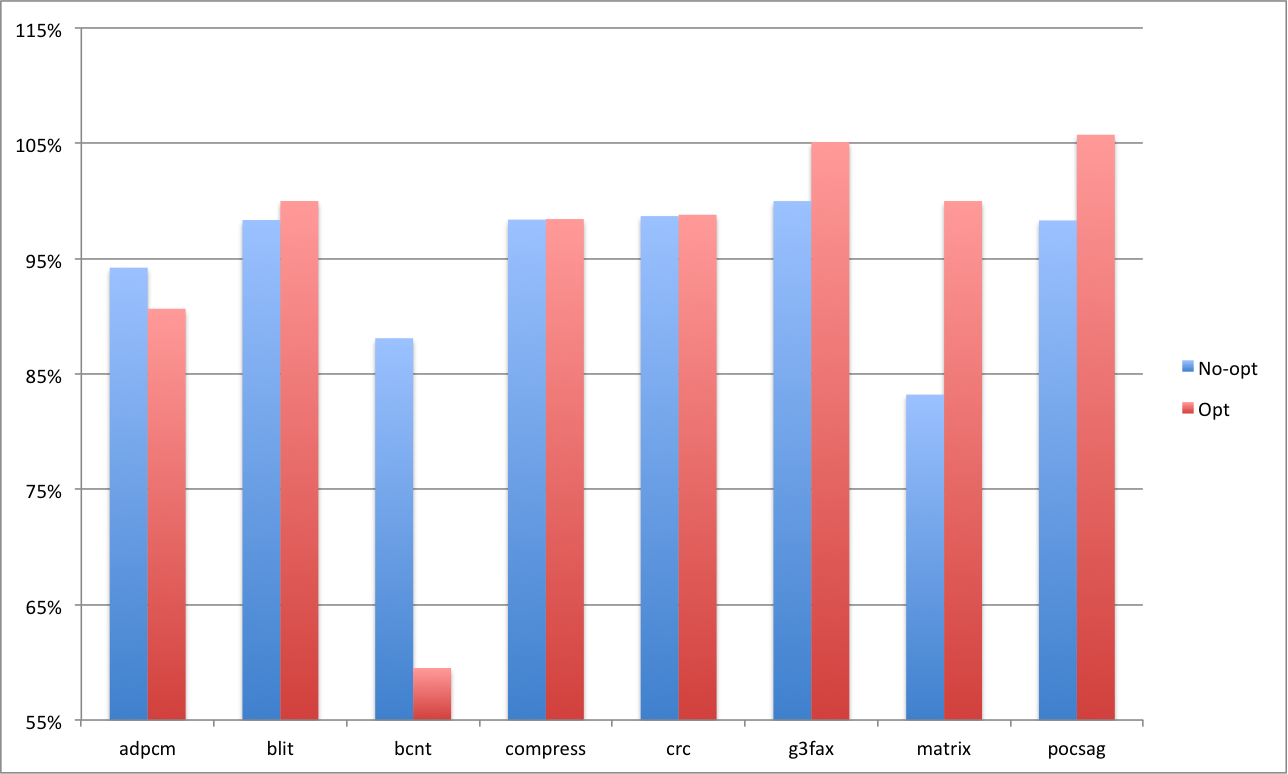
\includegraphics[width=0.8\textwidth]{5_results/img/rel_gen.png}
\caption{Generic-Regular performance}
\label{fig:rel_gen}
\end{figure}

Figure \ref{fig:rel_gen} shows that the optimization for generic binaries provides for more efficient generic binaries for most benchmarks. The \texttt{matrix} benchmark in particular shows excellent increase in performance. The \texttt{adpcm} benchmark however shows a significant decrease in performance. Closer inspection of the generated binaries shows that some benchmarks start spending a lot of time executing spill code to save registers to the stack. This is related to the optimization being to aggressive for \texttt{MachineBasicBlock} with a lot of virtual registers.

\begin{table}
  \centering
    \begin{tabular}{|l|r|r|r|}
    \hline
    \textbf{Benchmark} & \multicolumn{1}{|r|}{\textbf{Regular}} & \multicolumn{1}{|r|}{\textbf{No optimization}} & \multicolumn{1}{|r|}{\textbf{With optimization}} \\ \hline
	\texttt{adpcm} 		&  176.327 	&	 187.135 	&	 194.492 	\\ \hline
	\texttt{blit} 		&  100.328 	&	 102.007 	&	 100.325 	\\ \hline
	\texttt{compress} 	&  385.797 	&	 392.115 	&	 391.920 	\\ \hline
	\texttt{crc} 		&  107.528 	&	 108.950 	&	 108.820 	\\ \hline
	\texttt{matrix} 	&  51.238 	&	 61.572 	&	 51.238 	\\ \hline
	\texttt{ucbqsort} 	&  165.578 	&	 172.152 	&	 163.860 	\\ \hline
    \end{tabular}
  \caption{GCC-based compiler performance in ns}
  \label{tbl:GCC_perf}
\end{table}

\cite{Anthony-Brandon:2013jk} stated that performance should increase if more registers are used for generic binaries. The amount of different registers that are used by each benchmark have been tracked and are displayed in \ref{tbl:gen_regs}. The table shows that the optimization is able to increase the register usage for each benchmark. The \texttt{adpcm} benchmark already uses a large amount of registers and it is not possible to increase this by much. This probably causes the excessive spill code that is generated for this benchmark.

\begin{table}
  \centering
    \begin{tabular}{|l|r|r|r|}
    \hline
    \textbf{Benchmark} & \multicolumn{1}{|r|}{\textbf{Regular}} & \multicolumn{1}{|r|}{\textbf{No-opt}} & \multicolumn{1}{|r|}{\textbf{Opt}} \\ \hline
	\texttt{adpcm} 		&   49  &	49 & 	56 \\ \hline
	\texttt{blit} 		&   18  &	18 & 	33 \\ \hline
	\texttt{compress} 	&   27  &	27 & 	60 \\ \hline
	\texttt{crc} 		&   19  &	19 & 	27 \\ \hline
	\texttt{matrix} 	&   18 	&	18 & 	36 \\ \hline
	\texttt{ucbqsort} 	&   24  &	24 & 	31 \\ \hline
    \end{tabular}
  \caption{Register usage}
  \label{tbl:gen_regs}
\end{table}

\section{Conclusion}
In this section we have shown how the operation of the LLVM-based compiler has been verified and how well binaries execute that have been generated with the LLVM-based compiler.

The benchmarks and verifications have shown that the LLVM-based compiler still contains bugs. Not all benchmarks are able to execute using the Modelsim simulator but all benchmarks are able to execute using the XSTsim simulator. This indicates that there are probably scheduling issues in the assembly that is generated.

We have shown that the LLVM-based compiler exceeds the performance of the GCC-based compiler but the compiler is still outperformed by the HP-based compiler. As expected the HP-based compiler generates binaries that perform very well. This is probably related to the trace based scheduling techniques that are employed to extract a high level of ILP. In addition the HP-based compiler also performs certain optimizations that are not available to the LLVM-based compiler at \texttt{-O0}.

Additionally the benchmarks have also shown that the LLVM-based compiler is the only compiler able to generate correct code for all selected benchmarks. Surprisingly, even the HP-based compiler generates incorrect binaries for certain benchmarks. The code quality of the GCC-based compiler is bad with four benchmarks failing to execute.

Further we have also shown that the generic binary optimization allows generic binaries to operate at speeds that are nearly equel to the regular binaries. The generic binary optimization does introduce spill code in benchmarks that already use a large number of physical registers.
\acresetall
